\section{\toolname}\label{sec:liquidhaskell}
\begin{figure}[t!]
\centering
\captionsetup{justification=centering}
\noindent\makebox[\textwidth]{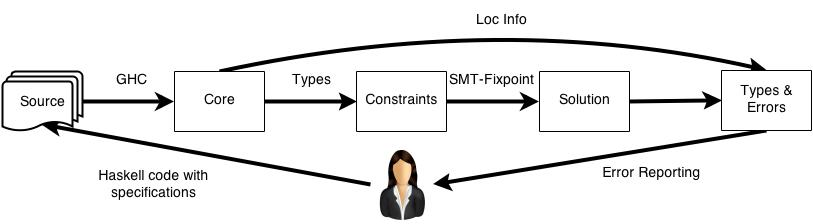
\includegraphics[width=\textwidth]{text/realworldhaskell/liquidHaskell}}
\caption{\toolname Workflow.}
	\label{fig:internals}
\end{figure}
% 
% link for workflow
% https://www.draw.io/#G0Bwp_mIorSVqJb2RENnNVWVlQTmc
%
We start with a short description of the \toolname workflow,
summarized in Figure~\ref{fig:internals} and continue with an 
example driven overview of how properties are specified
and verified using the tool. 

% \mypara{Usage} 
\mypara{Source}
\toolname can be run from the command-line\footnote{\url{https://hackage.haskell.org/package/liquidhaskell}}
or within a web-browser\footnote{\url{http://goto.ucsd.edu/liquid/haskell/demo/}}.
It takes as \emph{input}:
%
(1)~a single Haskell \emph{source} file with code and refinement
    type specifications including refined datatype definitions, 
    measures (\S~\ref{sec:tool:measures}), predicate and type 
    aliases, and function signatures;
%
(2)~a set of directories containing \emph{imported modules} 
    (including the \verb+Prelude+) which may themselves 
    contain specifications for exported types and functions; and
%
(3)~a set of predicate fragments called \emph{qualifiers},
    which are used to infer refinement types. This set is 
    typically empty as the default set of qualifiers extracted 
    from the type specifications suffices for inference.

\mypara{Core}
\toolname uses GHC to reduce the source to the Core IL~\cite{SulzmannCJD07}
and, to facilitate source-level error reporting, creates a map from Core 
expressions to locations in the Haskell source.

\mypara{Constraints}
Then, it uses the abstract interpretation framework of Liquid Typing~\cite{LiquidPLDI08}, 
modified to ensure soundness under lazy evaluation~\ref{chapter:refinedhaskell}
and extended with Abstract~\ref{chapter:abstractrefinements}
and Bounded~\ref{boundedrefinements} Refinement Types
and Refinement Reflection~\ref{refinementrflection},
to generate logical constraints from the Core IL.
     
\mypara{Solution}
Next, it uses a fixpoint algorithm (from~\citep{LiquidPLDI08})
combined with an SMT solver to solve the constraints, and hence 
infers a valid refinement typing for the program. 
%
\toolname can use any solver that implements the SMT-LIB2
standard~\cite{SMTLIB2}, including Z3~\citep{z3}, CVC4~\citep{CVC4}, and
MathSat~\citep{MathSat}.

 
\mypara{Types \& Errors}
% \NV{satisfiability and validity refer to different things here, 
% which is confusing...}
If the set of constraints is satisfiable, then \toolname outputs 
\textsc{Safe}, meaning the program is verified.
If instead, the set of constraints is not satisfiable, then \toolname
outputs \textsc{Unsafe}, and uses the invalid constraints to 
report refinement type errors at the \emph{source positions}
that created the invalid constraints, using the location 
information to map the invalid constraints to source positions.
%
In either case, \toolname produces as output a source map
containing the \emph{inferred} types for each program 
expression, which, in our experience, is crucial for 
debugging the code and the specifications.

%\mypara{Optional Typing}
%
\toolname is best thought of as an \emph{optional} type checker
for Haskell. By optional we mean that the refinements have \emph{no} 
influence on the dynamic semantics, which makes it easy to apply 
\toolname to \emph{existing} libraries.
%
To emphasize the optional nature of refinements and preserve 
compatibility with existing compilers, all specifications 
appear within comments of the form \verb|{-@ ... @-}|, 
which we omit below for brevity.

\subsection{Specifications}

A refinement type is a Haskell type where each component
of the type is decorated with a predicate from a (decidable)
refinement logic. We use the quantifier-free logic of equality, 
uninterpreted functions and linear arithmetic (QF-EUFLIA)~\cite{Nelson81}. 
For example,
%
\begin{code}
   {v:Int | 0 <= v && v < 100}
\end{code}
%
describes @Int@ values between @0@ and @100@.

\mypara{Type Aliases} For brevity and readability, it is often convenient 
to define abbreviations for particular refinement predicates and types.
For example, we can define an alias for the above predicate
%
\begin{code}
  predicate Btwn Lo N Hi = Lo <= N && N < Hi
\end{code}
%
and use it to define a \emph{type alias}
%
\begin{code}
  type Rng Lo Hi = {v:Int | Btwn Lo v Hi} 
\end{code}
%
We can now describe the above integers as @(Rng 0 100)@.

\mypara{Contracts} 
To describe the desired properties of a function, we need
simply refine the input and output types with predicates 
that respectively capture suitable pre- and post-conditions. 
For example,
%
\begin{code}
  range :: lo:Int -> hi:{Int | lo <= hi} 
        -> [(Rng lo hi)]
\end{code}
%
states that @range@ is a function that takes two @Int@s 
respectively named @lo@ and @hi@ and returns a list of @Int@s 
between @lo@ and @hi@. There are three things worth
noting.
%
First, we have binders to name the function's \emph{inputs} 
(\eg @lo@ and @hi@) and can use the binders inside the 
function's \emph{output}.
%
Second, the refinement in the \emph{input} type describes the 
\emph{pre-condition} that the second parameter @hi@ cannot 
be smaller than the first @lo@.
%
Third, the refinement in the \emph{output} type describes the
\emph{post-condition} that all returned elements are between 
the bounds of @lo@ and @hi@.


\subsection{Verification}\label{sec:tool:verification}

Next, consider the following implementation for @range@:
%
\begin{code}
  range lo hi 
    | lo <= hi  = lo : range (lo + 1) hi
    | otherwise = []
\end{code}
%
When we run \toolname on the above code, it reports an 
error at the definition of @range@. This is unpleasant! 
One way to debug the error is to determine what type has
been \emph{inferred} for @range@, \eg by hovering the 
mouse over the identifier in the web interface. 
In this case, we see that the output type is essentially:
%
\begin{code}
  [{v:Int | lo <= v && v <= hi}]
\end{code}
%
which indicates the problem. There is an \emph{off-by-one} 
error due to the problematic guard. If we replace the second @<=@ 
with a @<@ and re-run the checker, the function is verified.

\mypara{Holes} It is often cumbersome to specify the Haskell
types, as those can be gleaned from the regular type signatures 
or via GHC's inference. Thus, \toolname allows the user to leave 
holes in the specifications. Suppose @rangeFind@ has type 
%
\begin{code}
  (Int -> Bool) -> Int -> Int -> Maybe Int
\end{code}
%
where the second and third parameters define a range. 
We can give @rangeFind@ a refined specification:
%
\begin{code}
  _ -> lo:_ -> hi:{Int | lo <= hi} -> Maybe (Rng lo hi)
\end{code}
%
where the @_@ is the unrefined Haskell type for the 
corresponding position in the type.

\mypara{Inference} Next, consider the implementation
%
\begin{code}
  rangeFind f lo hi = find f $ range lo hi 
\end{code}
%$
where @find@ from @Data.List@ has the (unrefined) type
%
\begin{code}
  find :: (a -> Bool) -> [a] -> Maybe a
\end{code}
%
\toolname uses the abstract interpretation framework of 
Liquid Typing~\cite{LiquidPLDI08} to infer that the type
parameter @a@ of @find@ can be instantiated with @(Rng lo hi)@
thereby enabling the automatic verification of @rangeFind@.

Inference is crucial for automatically synthesizing types
for polymorphic instantiation sites -- note there is another
instantiation required at the use of the apply operator 
@dollar@ --  and to relieve the programmer of the tedium of %$
specifying signatures for all functions. 
%
Of course, for functions exported by the module,
we must write signatures to specify preconditions -- otherwise, 
the system defaults to using the trivial (unrefined) Haskell 
type as the signature \ie, checks the implementation assuming 
arbitrary inputs.

\subsection{Measures}\label{sec:tool:measures}
So far, the specifications have been limited to comparisons and 
arithmetic operations on primitive values. 
We use \emph{measure functions}, or just measures, to 
specify \emph{inductive properties} of algebraic data types. 
%
For example, we define a measure @len@ to write properties about the number
of elements in a list.
%
\begin{code}
  measure len :: [a] -> Int
  len []      = 0
  len (x:xs)  = 1 + (len xs)
\end{code}
%
Measure definitions are \emph{not} arbitrary Haskell code but a very 
restricted subset~\ref{sec:measures}.
Each measure has a single equation per constructor that defines the
value of the measure for that constructor. The right-hand side of the 
equation is a term in the restricted refinement logic. Measures are 
interpreted by generating refinement types for the corresponding 
data constructors.
%
For example, from the above, \toolname derives the 
following types for the list data constructors:
%
\begin{code}
  []  :: {v:[a]| len v = 0}
  (:) :: _ -> xs:_ -> {v:[a]| len v = 1 + len xs}
\end{code}
%
Here, @len@ is an \emph{uninterpreted function} in the refinement logic.
We can define multiple measures for a type; \toolname simply conjoins
the individual refinements arising from each measure to obtain a single
refined signature for each data constructor.

\mypara{Using Measures}
We use measures to write specifications about algebraic types. 
For example, we can specify and verify that: 
%
\begin{code}
  append :: xs:[a] -> ys:[a] 
         -> {v:[a]| len v = len xs + len ys}

  map    :: (a -> b) -> xs:[a] 
         -> {v:[b]| len v = len xs} 

  filter :: (a -> Bool) -> xs:[a] 
         -> {v:[a]| len v <= len xs}
\end{code}

\mypara{Propositions} 
%%In addition to allowing the specification of structural features like
%%lengths, heights and so on, 
Measures can be used to encode sophisticated 
invariants about algebraic data types.
%
To this end, the user can write a measure whose output has a special type 
@Prop@ denoting propositions in the refinement logic. For instance, we can
describe a list that contains a @0@ as:
%
\begin{code}
  measure hasZero :: [Int] -> Prop
  hasZero []      = false
  hasZero (x:xs)  = x == 0 || hasZero xs
\end{code}
%
We can then define lists containing a @0@ as:
%
\begin{code}
  type HasZero = {v : [Int] | hasZero v } 
\end{code}
%
Using the above, \toolname will accept 
%
\begin{code}
  xs0 :: HasZero 
  xs0 = [2,1,0,-1,-2]
\end{code}
%
but will reject
%
\begin{code}
  xs' :: HasZero 
  xs' = [3,2,1]
\end{code}



\subsection{Refined Data Types}

Often, we require that \emph{every} instance of a type satisfies some invariants. 
For example, consider a @CSV@ data type, that represents tables:
%
\begin{code}
  data CSV a = CSV { cols :: [String]
                   , rows :: [[a]]    }
\end{code}
%
% With \toolname we can enforce the invariant that for every @CSV@ table, 
% with a number of columns given by @dim@,
% each row has @dim@ elements,
% with the below refined data type definition
%%With \toolname we can enforce the invariant that every @CSV@ table 
%%has the number of columns given by @dim@, and that each row has 
%%@dim@ elements with a refined data type definition, such as:
With \toolname we can enforce the invariant that every row in a @CSV@ table
should have the same number of columns as there are in the header
%
\begin{code}
  data CSV a = CSV { cols :: [String]  
                   , rows :: [ListL a cols] }
\end{code}
%
using the alias
%
\begin{code}
  type ListL a X = {v:[a]| len v = len X}
\end{code}
%
A refined data definition is \emph{global} in that \toolname 
will reject any @CSV@-typed expression that does not respect 
the refined definition. For example, both of the below 
%
\begin{code}
  goodCSV = CSV [  "Month", "Days"] 
                [ ["Jan"  , "31"]
                , ["Feb   , "28"]
                , ["Mar"  , "31"] ]

  badCSV  = CSV [  "Month", "Days"] 
                [ ["Jan"  , "31"]
                , ["Feb   , "28"]
                , ["Mar"        ] ]
\end{code}
%
are well-typed Haskell, but the latter is rejected by \toolname.
%
Like measures, the global invariants are enforced by refining 
the constructors' types. 

\subsection{Refined Type Classes}\label{sec:type-classes}

Next, let us see how \toolname allows verification of
programs that use ad-hoc polymorphism via type classes.
%
While the implementation of each typeclass instance is 
different, there is often a common interface that 
all instances should satisfy.

\mypara{Class Measures}
As an example, consider the class definition
%
\begin{code}
  class Indexable f where
    size :: f a -> Int
    at   :: f a -> Int -> a
\end{code}
%
For safe access, we might require that @at@'s second 
parameter is bounded by the @size@ of the container.
To this end, we define a \emph{type-indexed} 
measure, using the @class measure@ keyword
%
\begin{code}
  class measure sz :: a -> Nat
\end{code}
%
Now, we can specify the safe-access precondition  
independent of the particular instances of @Indexable@:
%
\begin{code}
  class Indexable f where
    size :: xs:_ -> {v:Nat | v = sz xs}
    at   :: xs:_ -> {v:Nat | v < sz xs} -> a
\end{code}

\mypara{Instance Measures}
For each concrete type that instantiates a class, we require 
a corresponding definition for the measure. 
For example, to define lists as an instance of @Indexable@, 
we require the definition of the @sz@ instance for lists:
%
\begin{code}
  instance measure sz :: [a] -> Nat
  sz []     = 0
  sz (x:xs) = 1 + (sz xs)
\end{code}
%
Class measures work just like regular measures in that the above 
definition is used to refine the types of the list data constructors.
After defining the measure, we can define the type instance as:
%
\begin{code}
  instance Indexable [] where
    size []        = 0
    size (x:xs)    = 1 + size xs

    (x:xs) `at` 0  = x
    (x:xs) `at` i  = index xs (i-1)
\end{code}
%
\toolname uses the definition of @sz@ for lists to check that @size@ 
and @at@ satisfy the refined class specifications. 
% NV the dictionary relevant this were removed
% , and hence, that 
% the above creates a valid instance dictionary for @Indexable@.

\mypara{Client Verification}
At the clients of a type-class we use the refined 
types of class methods. Consider a client of @Indexable@s:
%
\begin{code}
  sum :: (Indexable f) => f Int -> Int
  sum xs = go 0 
    where
      go i | i < size xs = xs `at` i + go (i+1)
           | otherwise   = 0
\end{code}
%
\toolname proves that each call to @at@ is safe, by using the refined
class specifications of @Indexable@. 
Specifically, each call to @at@ is guarded by a check @i < size xs@
and @i@ is  increasing 
from 0, so \toolname proves that @xs `at` i@ will always be safe.

\begin{comment}
\subsection{Abstracting Refinements}

So far, all the specifications have used \emph{concrete} refinements. Often it is
useful to be able to \emph{abstract} the refinements that appear in a
specification. For example, consider a monomorphic variant of @max@
%
\begin{code}
  max     :: Int -> Int -> Int 
  max x y = if x > y then x else y
\end{code}
%
We would like to give @max@ a specification that lets us verify:
%
\begin{code}
  xPos  :: {v: _ | v > 0}
  xPos  = max 10 13

  xNeg  :: {v: _ | v < 0}
  xNeg  = max (-5) (-8)

  xEven :: {v: _ | v mod 2 == 0} 
  xEven = max 4 (-6)
\end{code}
%
To this end, \toolname allows the user to \emph{abstract refinements} over
types~\cite{vazou13}, for example by typing @max@ as:
%
\begin{code}
 max :: forall <p :: Int -> Prop>. 
          Int<p> -> Int<p> -> Int<p>
\end{code}
%
The above signature states that for any refinement @p@, if the two
inputs of @max@ satisfy @p@ then so does the output. \toolname uses
Liquid Typing to automatically instantiate @p@ with suitable concrete
refinements, thereby checking @xPos@, @xNeg@, and @xEven@.


\mypara{Dependent Composition}
Abstract refinements turn out to be a surprisingly expressive and 
useful specification mechanism. For example, consider the function 
composition operator:
%
\begin{code}
  (.) :: (b -> c) -> (a -> b) -> a -> c
  (.) f g x = f (g x)  
\end{code}
%
Previously, it was not possible to check, \eg that:
%
\begin{code}
  plus3 :: x:_ -> {v:_ | v = x + 3}
  plus3 = (+ 1) . (+ 2)
\end{code}
%
as the above required tracking the dependency between @a@, @b@ and @c@,
which is crucial for analyzing idiomatic Haskell.
With abstract refinements, we can give the @(.)@ operator the type:
%
\begin{code}
  (.) :: forall < p :: b -> c -> Prop
                , q :: a -> b -> Prop>.
           f:(x:b -> c<p x>) 
        -> g:(x:a -> b<q x>) 
        -> y:a 
        -> exists[z:b<q y>].c<p z>
\end{code}
%
which gets automatically instantiated at usage sites, allowing \toolname
to precisely track invariants through the use of the ubiquitous 
higher-order operator.

\mypara{Dependent Pairs}
Similarly, we can abstract refinements over the definition of datatypes.
% Similarly, we can abstract refinements over the definition of datatypes.
For example, we can express dependent pairs in \toolname by refining the 
definition of tuples as:
%
\begin{code}
  data Pair a b <p :: a -> b -> Prop> 
    = Pair { fst :: a, snd :: b<p fst>}
\end{code}
%
That is, the refinement @p@ relates the @snd@ element with the @fst@.
Now we can define increasing and decreasing pairs
%
\begin{code}
  type IncP = Pair <{\x y -> x < y}> Int Int
  type DecP = Pair <{\x y -> x > y}> Int Int
\end{code}
%
and then verify that:
%
\begin{code}
  up :: IncP
  up = Pair 2 5
  
  dn :: DecP
  dn = Pair 5 2
\end{code}
%
Now that we have a bird's eye view of the various specification mechanisms
supported by \toolname, let us see how we can profitably apply them to
statically check a variety of correctness properties in real-world codes.
\end{comment}
%%% Local Variables: 
%%% mode: latex
%%% TeX-master: "main"
%%% End: 
